%%%%%%%%%%%%%%%%%%%%%%%%%%%%%%%%%%%%%%%%%%%
%
% From a template maintained at https://github.com/jamesrobertlloyd/cbl-tikz-poster
%
% Code near the top should be fairly standard and not need to be changed
%  - except for the document class
% Code lower down is more likely to be customised
%
%%%%%%%%%%%%%%%%%%%%%%%%%%%%%%%%%%%%%%%%%%%

%%%%%%%%%%%%%%%%%%%%%%%%%%%%%%%%%%%%%%%%%%%
%
% Document class
%
% Change this if you want a different size / orientation poster etc
%
%%%%%%%%%%%%%%%%%%%%%%%%%%%%%%%%%%%%%%%%%%%

%\documentclass[portrait,a0,final]{a0poster}
\documentclass[portrait,a0,final]{a0poster}

%%%%%%%%%%%%%%%%%%%%%%%%%%%%%%%%%%%%%%%%%%%
%
% 'Basic' packages
%
% TODO - Almost certainly some are unnecessary - feel free to remove nonstandard
% packages if you think it is a good idea not to always have them
%
%%%%%%%%%%%%%%%%%%%%%%%%%%%%%%%%%%%%%%%%%%%

\usepackage{multicol}
\usepackage{color}
\usepackage{shadow}
\usepackage{morefloats}
%\usepackage{cite}
\usepackage[pdftex]{graphicx}
\usepackage{rotating}
\usepackage{amsmath, amsthm, amssymb, bm}
\DeclareMathOperator*{\argmax}{arg\,max}
\DeclareMathOperator*{\argmin}{arg\,min}
\usepackage{array}
\usepackage{nth}
\usepackage[square,numbers]{natbib}
\usepackage{booktabs}
\usepackage[table,xcdraw]{xcolor}
\usepackage{float}
%\usepackage{subfig}
%\usepackage{svg}
%\usepackage{wrapfig}
%\usepackage[a0paper,pass]{geometry}
\usepackage{graphicx,array}
%%%%%%%%%%%%%%%%%%%%%%%%%%%%%%%%%%%%%%%%%%%
%
% TIKZ packages and common definitions
%
% Add extra things as per your tikz needs
%
%%%%%%%%%%%%%%%%%%%%%%%%%%%%%%%%%%%%%%%%%%%

\usepackage{picins}
\usepackage{tikz}
\usetikzlibrary{shapes.geometric,arrows,chains,matrix,positioning,scopes,calc}
\tikzstyle{mybox} = [draw=white, rectangle]

%%%%%%%%%%%%%%%%%%%%%%%%%%%%%%%%%%%%%%%%%%%
%
% myfig
%
% \myfig - replacement for \figure
% necessary, since in multicol-environment 
% \figure won't work        
%                 
%%%%%%%%%%%%%%%%%%%%%%%%%%%%%%%%%%%%%%%%%%%

\newcommand{\myfig}[3][0]{
\begin{center}
  \vspace{1.5cm}
  \includegraphics[width=#3\hsize,angle=#1]{#2}
  \nobreak\medskip
\end{center}}

%%%%%%%%%%%%%%%%%%%%%%%%%%%%%%%%%%%%%%%%%%%
%
% mycaption                
%
% \mycaption - replacement for \caption
% necessary, since in multicol-environment \figure and
% therefore \caption won't work
%
%%%%%%%%%%%%%%%%%%%%%%%%%%%%%%%%%%%%%%%%%%%

%\newcounter{figure}
\setcounter{figure}{1}
\newcommand{\mycaption}[1]{
  \vspace{0.5cm}
  \begin{center}
    {#1}
  \end{center}
  \vspace{0.5cm}
  \stepcounter{figure}
}

\setcounter{table}{1}
\newcommand{\mytablecaption}[1]{
  \vspace{0.5cm}
  \begin{center}
    \begin{quote}
        {#1}
    \end{quote}    
  \end{center}
  \vspace{1cm}
  \stepcounter{table}
}

\newcommand{\cwicaption}[1]{
  %\vspace{0.5cm}
  \begin{quote}
    {{\sc Figure} \arabic{figure}: #1}
  \end{quote}
  %\vspace{1cm}
  \stepcounter{figure}
}

%%%%%%%%%%%%%%%%%%%%%%%%%%%%%%%%%%%%%%%%%%%
%
% Some standard colours
%
%%%%%%%%%%%%%%%%%%%%%%%%%%%%%%%%%%%%%%%%%%%

\definecolor{camlightblue}{rgb}{0.601 , 0.8, 1}
\definecolor{camdarkblue}{rgb}{0, 0.203, 0.402}
\definecolor{camred}{rgb}{1, 0.203, 0}
\definecolor{camyellow}{rgb}{1, 0.8, 0}
\definecolor{lightblue}{rgb}{0, 0, 0.80}
\definecolor{white}{rgb}{1, 1, 1}
\definecolor{whiteblue}{rgb}{0.80, 0.80, 1}
\definecolor{cwired}{rgb}{0.803,0.0,0.227}

%%%%%%%%%%%%%%%%%%%%%%%%%%%%%%%%%%%%%%%%%%%
%
% Some look and feel definitions
%
%%%%%%%%%%%%%%%%%%%%%%%%%%%%%%%%%%%%%%%%%%%

\setlength{\columnsep}{0.03\textwidth}
\setlength{\columnseprule}{0.0018\textwidth}
\setlength{\parindent}{0.0cm}

%%%%%%%%%%%%%%%%%%%%%%%%%%%%%%%%%%%%%%%%%%%
%
% \mysection - replacement for \section*
% 
% Puts a pretty box around some text
% TODO - any other thoughts for what this box should look like
%
%%%%%%%%%%%%%%%%%%%%%%%%%%%%%%%%%%%%%%%%%%%

\tikzstyle{mysection} = [rectangle, 
						draw=none, 
						shade, 
						outer color=cwired,
						inner color=cwired,
						text width=0.95\columnwidth,
						text centered,
						rounded corners=20pt,
						minimum height=0.11\columnwidth]

\newcommand{\mysection}[1]
{
\begin{center}
  \begin{tikzpicture}
    \node[mysection,white] {\sffamily\bfseries\LARGE#1};
  \end{tikzpicture}
\end{center}
}



%%%%%%%%%%%%%%%%%%%%%%%%%%%%%%%%%%%%%%%%%%%
%
% Set the font
%
% TODO - Not sure what a canonical choice is - feel free to modify
%
%%%%%%%%%%%%%%%%%%%%%%%%%%%%%%%%%%%%%%%%%%%

\renewcommand{\familydefault}{cmss}
\sffamily

%%%%%%%%%%%%%%%%%%%%%%%%%%%%%%%%%%%%%%%%%%%
%
% Poster environment
%
% Centres everything and can be used to define the width of the content
%
%%%%%%%%%%%%%%%%%%%%%%%%%%%%%%%%%%%%%%%%%%%

\newenvironment{poster}{
  \begin{center}
  \begin{minipage}[c]{0.95\textwidth}
}{
  \end{minipage} 
  \end{center}
}

%%%%%%%%%%%%%%%%%%%%%%%%%%%%%%%%%%%%%%%%%%%
%
% This is probably a good place to put content specific packages and definitions
%
%%%%%%%%%%%%%%%%%%%%%%%%%%%%%%%%%%%%%%%%%%%

%%%%%%%%%%%%%%%%%%%%%%%%%%%%%%%%%%%%%%%%%%%
%
% The document environment starts here
%
%%%%%%%%%%%%%%%%%%%%%%%%%%%%%%%%%%%%%%%%%%%

\begin{document}
%%%%%%%%%%%%%%%%%%%%%%%%%%%%%%%%%%%%%%%%%%%
%
% Begin the poster environment - centres things and potentially changes the width
%
%%%%%%%%%%%%%%%%%%%%%%%%%%%%%%%%%%%%%%%%%%%

\begin{poster}

%%%%%%%%%%%%%%%%%%%%%%%%%%%%%%%%%%%%%%%%%%%
%
% Potentially add some space at the top of the poster
%
%%%%%%%%%%%%%%%%%%%%%%%%%%%%%%%%%%%%%%%%%%%

\vspace{1\baselineskip}

%%%%%%%%%%%%%%%%%%%%%%%%%%%%%%%%%%%%%%%%%%%
%
% Draw the header as a TIKZ picture
%
% Using TIKZ to allow for easy alignment
%
%%%%%%%%%%%%%%%%%%%%%%%%%%%%%%%%%%%%%%%%%%%

\begin{center}
\begin{tikzpicture}[x=0.5\textwidth]
    % Dummy nodes at edges for spacing
    % TODO - a better way?
    \node at (+1, 0) {};    
    \node at (-1, 0) {};
    % Set the size of the badges
    \def \badgeheight {0.08\textwidth}
    % Title text
    \node[inner sep=0,text width=0.8\textwidth,text centered,font=\Huge] (Title) at (-0.3,0) 
    {
        {\sffamily\veryHuge \textbf{Causal Dynamic Time Lag : What? and When?}}\\
        {\sffamily\Huge \underline{Mandar Chandorkar}$^{1,2}$, Cyril Furthlener$^2$, 
        Bala Poduval$^3$, 
        Enrico Camporeale$^1$, 
        Michele Sebag$^2$}\\
        \vspace{-0.2\baselineskip}
        {\sffamily\LARGE 1 Multiscale Dynamics, CWI, Amsterdam, 
        2 TAU, INRIA Paris-Saclay 
        3 UNH, New Hampshire}\\
        \vspace{-0.3\baselineskip}
        {\sffamily\LARGE www.mlspaceweather.org}
    };
    % Cambridge badge
    \node [mybox] (CWI Logo) at (-1.2, -0.4) {
        
\includegraphics[height=0.05\textwidth]{cwi-logo.png}
    };
    % CBL badge
    \node [mybox] (Inria logo) at (+0.54, -0.4) {
        
\includegraphics[height=0.05\textwidth]{inria-logo.jpg}
    };
\end{tikzpicture}
\end{center}

%%%%%%%%%%%%%%%%%%%%%%%%%%%%%%%%%%%%%%%%%%%
%
% Spacing between title and main body
%
%%%%%%%%%%%%%%%%%%%%%%%%%%%%%%%%%%%%%%%%%%%

%\vspace{.8\baselineskip}

%%%%%%%%%%%%%%%%%%%%%%%%%%%%%%%%%%%%%%%%%%%
%
% Columns environment
%
%%%%%%%%%%%%%%%%%%%%%%%%%%%%%%%%%%%%%%%%%%%



%%%%%%%%%%%%%%%%%%%%%%%%%%%%%%%%%%%%%%%%%%%
%
% Start of content
%
%%%%%%%%%%%%%%%%%%%%%%%%%%%%%%%%%%%%%%%%%%%

\large

%\begin{tabular}{lr}
%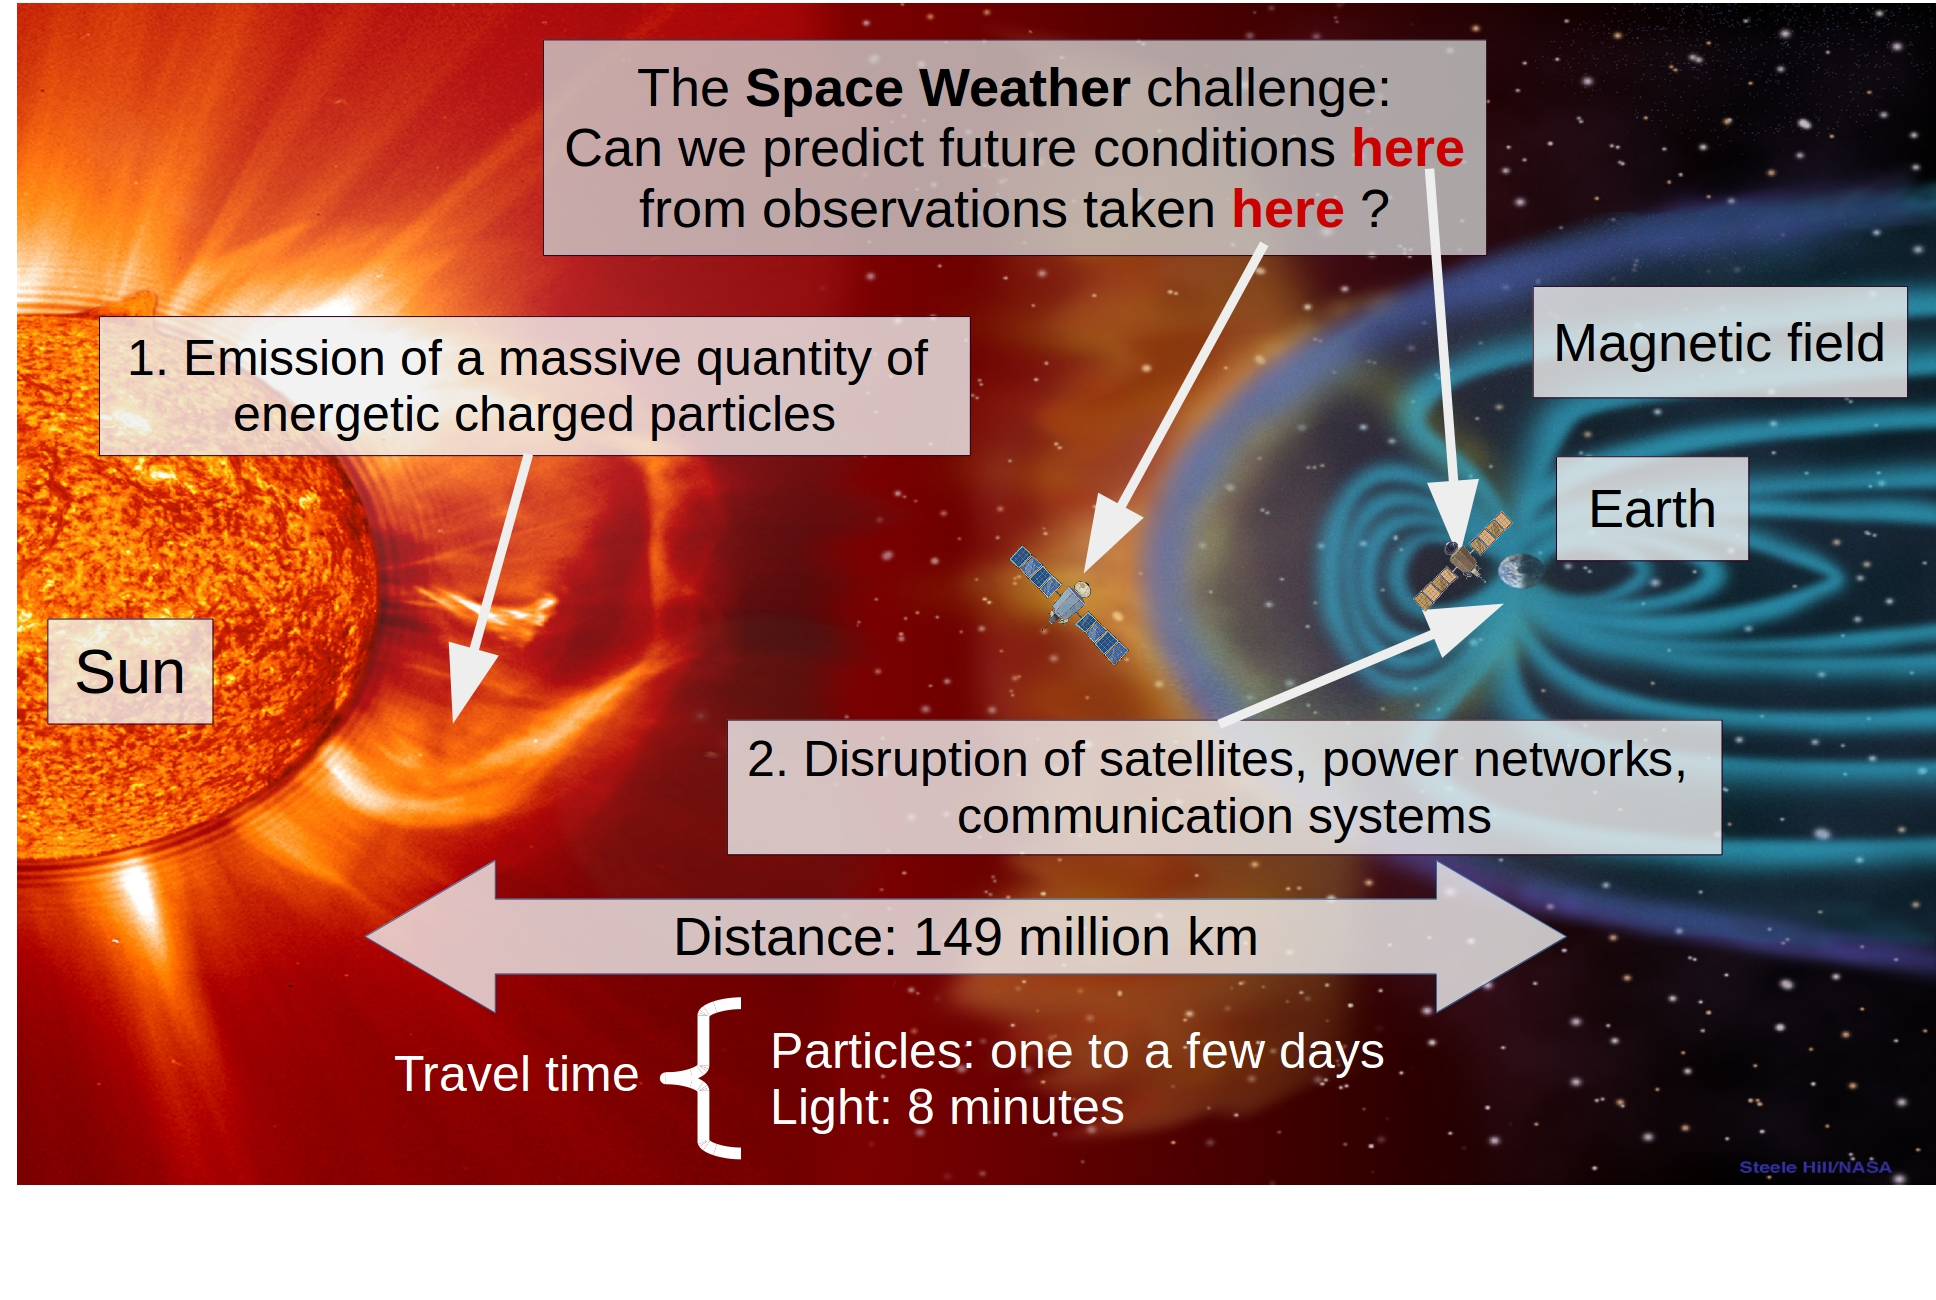
\includegraphics[width=0.48\hsize]{magnetosphere_shifted} &
%\mycaption{Space Weather Drivers and Dynamics}
%\hspace{9cm}
%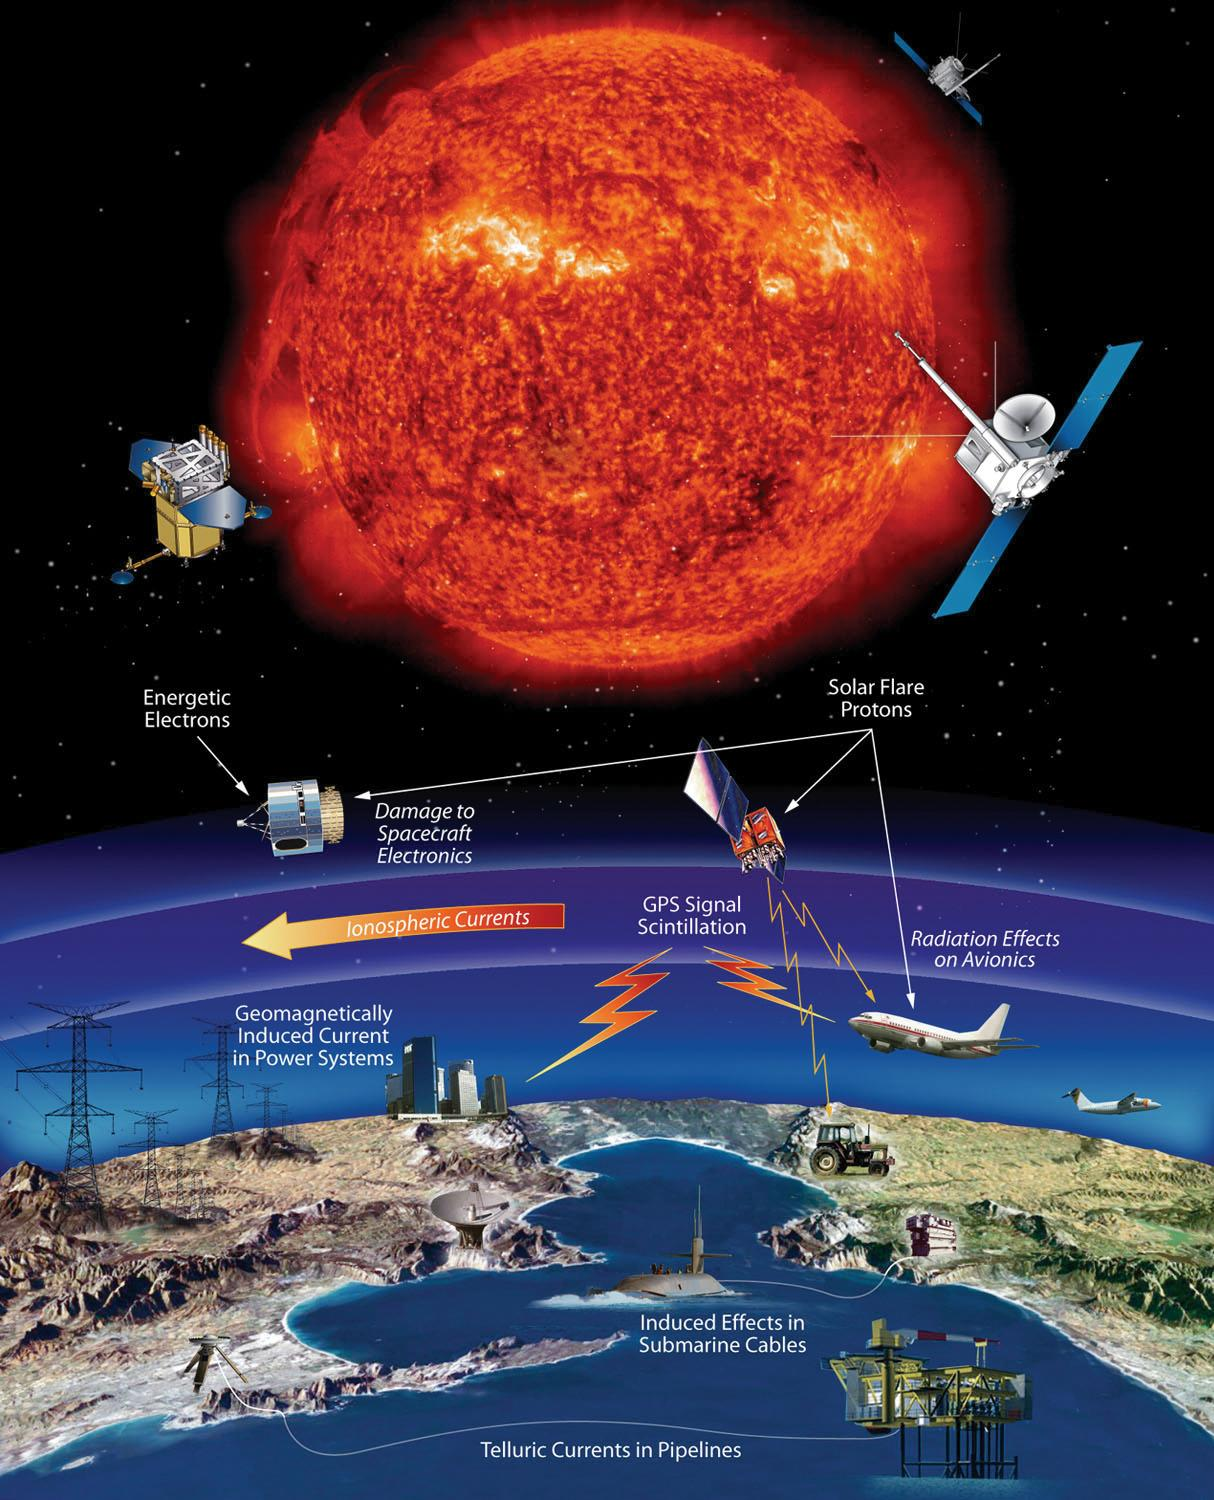
\includegraphics[width=0.28\hsize]{nasa-space-weather}\\
%\end{tabular}

\begin{multicols}{2}


\mysection{Sun-Earth System}

\myfig{magnetosphere}{0.65}

The Sun ejects charged energetic particles, known as the \emph{solar wind}, into the surrounding space. Depending on the nature of activity on the Sun, its effects are observed near the Earth after some time delay, which is variable and uncertain.

\vspace{0.5\baselineskip}
\mysection{Causal Time Lag \& Propagation Time}
\myfig{GrangerCausalityIllustration}{0.65}

Learning the the time delay between causes and effects, from data, is an important and challenging problem. We call this problem \emph{Causal Dynamic Time Lag} and formulate it as follows.
%\vfill
%\columnbreak

\begin{enumerate}
\item \textbf{Inputs}: Two time series, the causes $x(t)$ and the observed effects $y(t)$
\item \textbf{Outputs}: A function $f: \mathcal{X}  \rightarrow \mathbb{R}$ which maps each input pattern $x(t_1)$ to an output $y(t_2)$, and $g:\mathcal{X}  \rightarrow \mathbb{R}^{+}$ which maps the time delay between the input and output patterns $t_2 = t_1 + g(x(t_1))$.
\end{enumerate}

\begin{align}
y(t + \Delta(t)) & = f[x(t)]\label{eq:pb1}\\
\Delta(t) & = g[x(t)]\label{eq:pb2} 
\end{align}

\mysection{Proposed Solution}

Define for every time step $t$, a \emph{causal time window} $[t+\ell, t+\ell+h)$. 
\vspace{0.4\baselineskip}

\textbf{Inputs}: Time series $x(t) \in \mathbb{R}^{n}$ \vspace{0.5\baselineskip}

\textbf{Model Outputs}: 
\begin{enumerate}
\item Targets $[\hat{y}(t+\ell), \cdots, \hat{y}(t+\ell+h-1)]$
\item Time Lag Probabilities $[\hat{p}(t+\ell), \cdots, \hat{p}(t+\ell+h-1)], \ \sum^{h-1}_{i = 0}{\hat{p}_{i}} = 1$
\end{enumerate}

\vspace{0.4\baselineskip}

\textbf{Predictions}: For an input $x(t)$, predict the target $\hat{y}(t + \ell + i^{*})$ corresponding to the most probable propagation time $i^{*} = \argmin_{i}{\hat{p}_i(x(t))}$

\vspace{0.4\baselineskip}

\textbf{Architecture}: The proposed model architecture takes the form of a neural network model as seen below.
\myfig{network}{0.65}

\textbf{Model Training}: In order to build time lag based models, we must devise an objective/loss function which favours.

\begin{enumerate}
    \item Accurate predictions for time window $y(t+\ell), \cdots, y(t+\ell+h-1)$
    \item Learning the time lag structure.
\end{enumerate}


The neural network parameters are updated using gradient based minimization of equation \ref{eq:loss}.


\begin{equation}\label{eq:loss}
\begin{aligned}
\mathcal{L}(y^{(1:M)}, \hat{y}^{(1:M)}, \hat{p}^{(1:M)}) = & \lambda_1 \frac{1}{2M} \sum_{i,m}{(y^{(m)}_{i} - \hat{y}^{(m)}_{i})^2 (1 + \hat{p}^{(m)}_i)} \\ 
+ &\lambda_2 \frac{1}{M} \sum_{i,m}{\hat{p}^{m}_{i} log \left( \frac{\hat{p}^{m}_{i}}{\widetilde{p}_{i}}\right )}
\end{aligned}
\end{equation}

The quantity $\widetilde{p}_i, i \in {1, \cdots, h}$ represents some \emph{apriori} knowledge of the propagation time distribution. In the experiments run here, we choose $\widetilde{p}_i = 1/h$.




\vspace{0.5\baselineskip}

\mysection{Experiments}

\textbf{Data Generation}: Time series $x(t) \in \mathbb{R}^8$, of size $4000$ (one copy for training and another for test), using \emph{Stochastic Langevin Dynamics} as shown in equation \ref{eq:data}.

\begin{align}
 x(t+1) &= (1 - \tau) x(t) + \mathcal{N}(0, \sigma^2) \label{eq:data}\\
 y(t+\Delta(t)) &= \alpha ||x(t)||^2 \label{eq:outputs}
\end{align}

\begin{enumerate}
\item \textbf{Problem I} Constant Velocity $\alpha ||x(t)||^2 + c$; Fixed Distance $d$: 
\newline $\Delta(t) = d/(\alpha ||x(t)||^2 + c),\ \alpha = \frac{100}{8},\ d = 1000,\ c = 40$

\item \textbf{Problem II} Constant Acceleration $a$; Fixed Distance $d$: 
\newline $\Delta(t) = (\sqrt{\alpha^2||x(t)||^4 + 2ad} - \alpha||x(t)||^2)/a,\ \alpha = \frac{50}{8},\ a = 5,\ d = 1000$

\end{enumerate}


\myfig{exp2_scatter_v_tl}{0.4}

\mycaption{\textbf{Problem I}: Output vs Propagation time relationship}


\myfig{exp3_scatter_v_tl}{0.4}

\mycaption{\textbf{Problem II}: Output vs Propagation time relationship}

\begin{center}
\begin{tabular}{p{0.2\linewidth}p{0.2\linewidth}p{0.2\linewidth}p{0.2\linewidth}}
\hline
\noalign{\smallskip}
\multicolumn{4}{c}{Predictive Performance: Time Lag} \\
\hline
Problem  &  M.A.E  &  Correlation & Data Range \\
\noalign{\smallskip}
\hline
\noalign{\smallskip}
I & $0.763$ & $0.899$ & $[1, 16]$\\
II & $1.492$ & $0.934$ & $[1, 16]$ \\
\noalign{\smallskip}
\hline
\end{tabular}
\end{center}

\begin{center}
\begin{tabular}{p{0.2\linewidth}p{0.2\linewidth}p{0.2\linewidth}p{0.2\linewidth}}
\hline
\noalign{\smallskip}
\multicolumn{4}{c}{Predictive Performance: Output} \\
\hline
Problem  &  M.A.E  &  Correlation & Data Range\\
\noalign{\smallskip}
\hline
\noalign{\smallskip}
I & $20.186$ & $0.983$ & $[60, 575]$ \\
II & $16.204$ & $0.980$ & $[100, 700]$  \\
\noalign{\smallskip}
\hline
\end{tabular}
\end{center}


%\vspace{\baselineskip}
\mysection{Future Work}
\begin{enumerate}
    \item Application of our proposed method to the problem of predicting solar wind propagation time using solar images. 
    \item Manuscript (under review) AISTATS 2019\\
\end{enumerate}
    %\vspace{.5\baselineskip}
    %Ref: Chandorkar, Camporeale, Wing \emph{Gaussian Processes Autoregressive Models for Forecasting the Disturbance Storm Time Index}

\end{multicols}

\end{poster}

\end{document}
